%====================================================================%
%                  BLOIS.TEX                                         %
%====================================================================%
\documentclass{blois}

\usepackage{lineno}
%\linenumbers

% A useful Journal macro
\def\Journal#1#2#3#4{{#1} {\bf #2}, #3 (#4)}

% Some useful journal names
\def\NCA{\em Nuovo Cimento}
\def\NIM{\em Nucl. Instrum. Methods}
\def\NIMA{{\em Nucl. Instrum. Methods} A}
\def\NPB{{\em Nucl. Phys.} B}
\def\PLB{{\em Phys. Lett.}  B}
\def\PRL{\em Phys. Rev. Lett.}
\def\PRD{{\em Phys. Rev.} D}
\def\ZPC{{\em Z. Phys.} C}

% Some other macros used in the sample text
\def\st{\scriptstyle}
\def\sst{\scriptscriptstyle}
\def\mco{\multicolumn}
\def\epp{\epsilon^{\prime}}
\def\vep{\varepsilon}
\def\ra{\rightarrow}
\def\ppg{\pi^+\pi^-\gamma}
\def\vp{{\bf p}}
\def\ko{K^0}
\def\kb{\bar{K^0}}
\def\al{\alpha}
\def\ab{\bar{\alpha}}
\def\be{\begin{equation}}
\def\ee{\end{equation}}
\def\bea{\begin{eqnarray}}
\def\eea{\end{eqnarray}}
\def\CPbar{\hbox{{\rm CP}\hskip-1.80em{/}}}
%temp replacement due to no font
%%%%%%%%%%%%%%%%%%%%%%%%%%%%%%%%%%%%%%%%%%%%%%%%%%
%                                                %
%    BEGINNING OF TEXT                           %
%                                                %
%%%%%%%%%%%%%%%%%%%%%%%%%%%%%%%%%%%%%%%%%%%%%%%%%%
%\newcommand{\Photo}{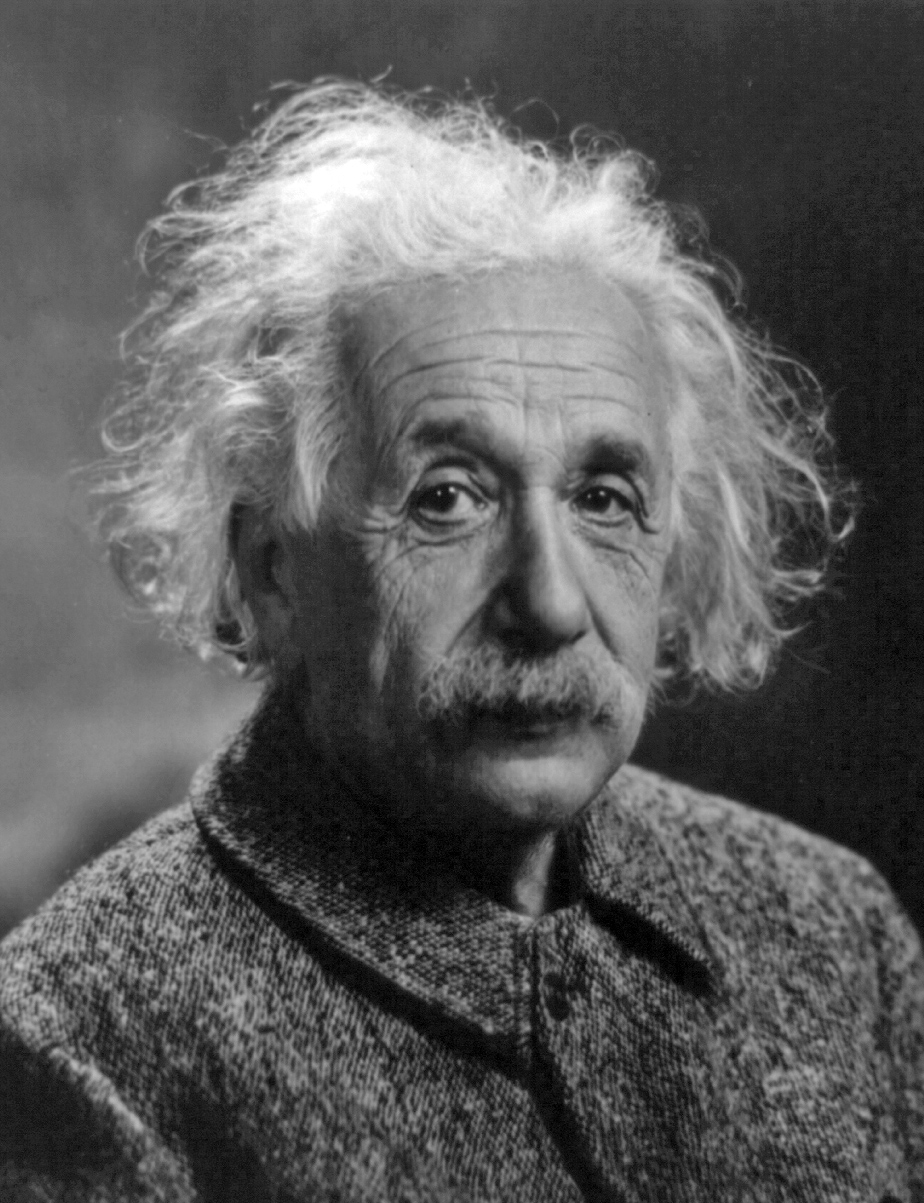
\includegraphics[height=35mm]{mypicture}}
\begin{document}
\vspace*{4cm}
\title{Searches for an extended Higgs boson sector at CMS}

\author{Khawla Jaffel\\
on behalf of the CMS Collaboration}
\address{UCLouvain Center for Cosmology, \\
Particle Physics and Phenomenology, (Belgium).}

\maketitle\abstracts{
    The existence of the final building block of the Standard Model (SM) was confirmed by the
discovery of the Higgs boson by the CMS and the ATLAS detectors in 2012. This
discovery ultimately crowned the SM as the most successful explanation of
particle physics ever to be achieved, but this theory still falls short of providing a unified
description of the fundamental interactions.
To remedy the incompleteness of the SM, many scenarios of physics Beyond the Standrd Model (BSM) were proposed of particular interest to better understand the behavior of nature at high energies, in the hope of finding hints of what may lie ahead of the standard model.
This report, is a brief overview of the most recent full run 2 CMS searches in the context of an extended Higgs boson sector.
}
%%%%%%%%%%%%%%%%%%%%%%%%%%%%%%%%%%%%%%%%%%%%%%%%%%%%%%%%%%%%%%%%%%%%%%%%%%%
\section{Introduction}
    The discovery of a Higgs boson with a mass around 125 GeV at the LHC in 2012~\cite{20121,201230}
has shifted the focus of the CMS and ATLAS experiments on measurements of the properties of the newly
discovered Higgs particle. To date, all measurements agree reasonably well with the Standard
Model (SM) across nine orders of magnitude as shown in the summary of the standard model cross section predictions and corresponding measurements by the CMS collaboration~\cite{Collaboration_2008} in Fig.~\ref{fig:mes}. There are no requirements for the Higgs sector to be minimal. There are still a few questions in physics that the SM fails to explain.  For example, the SM provides no dark matter candidate and no
explanation for the matter–antimatter asymmetry in the universe, nor the ability to include the gravitational interaction within the model. %Again, the theory of the standard model is built based on gauge symmetry and expect it to be broken through strong interactions which govern quantum chromodynamics (QCD), but no such asymmetry has been found.

\begin{figure}[!htbp]
    \begin{center}
        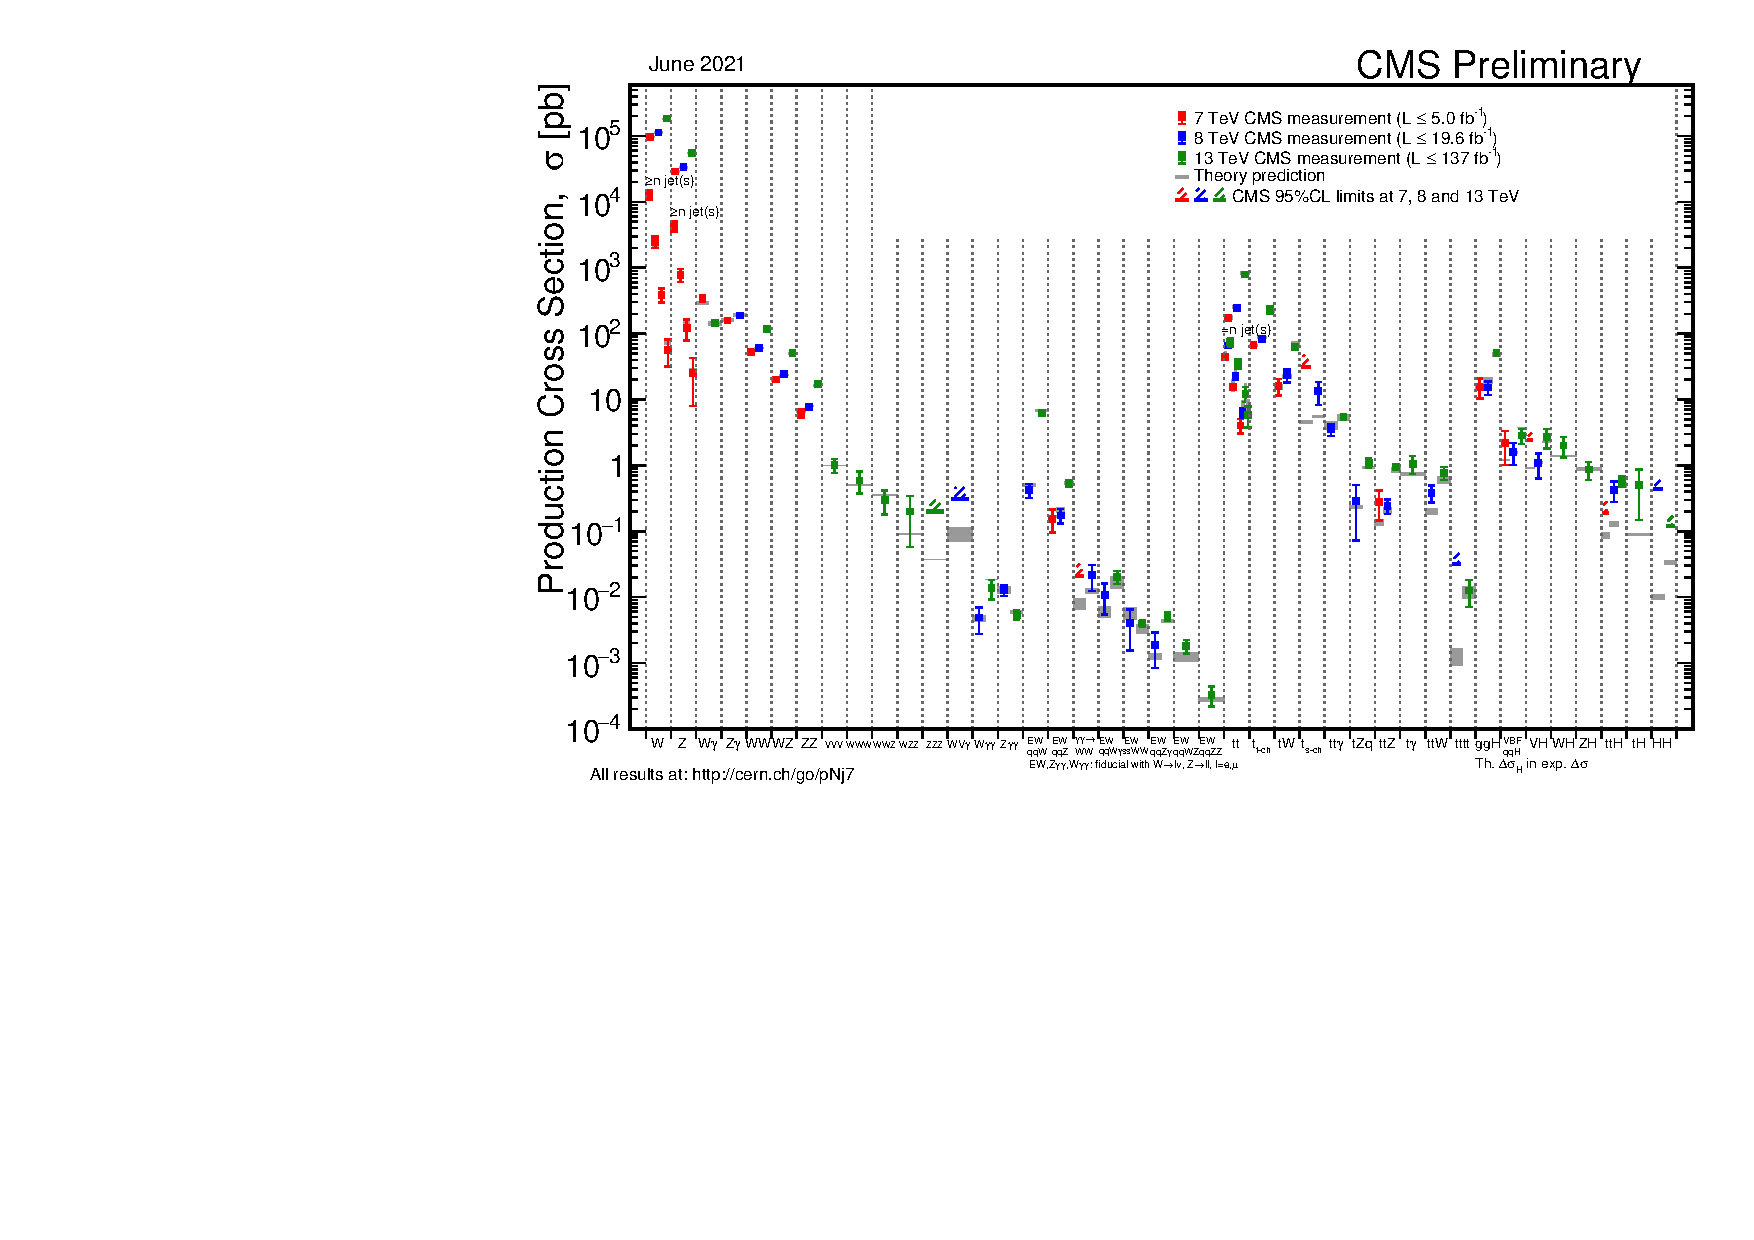
\includegraphics[width=0.7\textwidth]{SigmaNew_v0.pdf}
        \caption{
            Summary of the cross section measurements of Standard Model processes~\protect\cite{CMS:xsc_mes}.
        }
        \label{fig:mes}
    \end{center}
\end{figure}

Extended Higgs sectors address these deficiencies via numerous theoretical scenarios. 
Models with extended Higgs sectors provide very interesting benchmarks, from the existence of charged Higgs bosons to CP-violating scalars that can be probed by the experimental collaborations at the LHC.
The Two-Higgs-Doublet-Model (2HDM) for example is one of the simplest extensions of the standard model, and is built by simply adding one more scalar doublet to the SM field content while keeping the Lagrangian invariant under the same symmetries. It was proposed as a means to provide an extra source of CP-violation~\cite{Lee:1973iz}. 

In this manuscript, we will focus on the ongoing searches and recently published searches using the CMS detector~\cite{CMS:2008xjf} in the context of the extended Higgs boson sector.
%%%%%%%%%%%%%%%%%%%%%%%%%%%%%%%%%%%%%%%%%%%%%%%%%%%%%%%%%%%%%%%%%%%%%%%%%%%
\section{Neutral Higgs searches}
In the minimal supersymmetric extension of the SM (MSSM)~\cite{ELLWANGER20101} one more $SU(2)$ doublet of complex scalar fields is introduced with respect to the SM, leading to the prediction of two charged and three neutral Higgs bosons, one of which can be associated with the observed Higgs h(125 GeV). In an attempt to explain why the $\mu$ parameter in the superpotential term  $\mu H_{u} H_{d}$ is at the electroweak scale, denoted as the "$\mu$-problem" of the MSSM~\cite{KIM1984150}, a further extension of the MSSM by one additional complex scalar field S is introduced, resulting in the Next-to-Minimal Supersymmetric Standard Model (NMSSM).

\subsection{Search for light Higgs bosons from supersymmetric cascade decays}
In this section we describe a recent search using full LHC run 2 proton-proton collision data, at a center-of-mass energy of 13 TeV, corresponding to an integrated luminosity of 137 $fb^{-1}$, is looking for a pair of boosted light Higgs bosons ($H_{1}$) produced in supersymmetric cascade decays~\cite{CMS-PAS-HIG-20-018}. The results are interpreted in the context of NMSSM extension of the SM~\cite{ELLWANGER20101}, where a low-mass singlino leads to multi-step squark and gluino decays that can predominantly end with a boosted singlet-like $H_{1}$ boson and a low-momentum singlino-like neutralino as displayed in Fig.~\ref{fig:susy_diagram}.

\begin{figure}[!htb]
    \begin{center}
        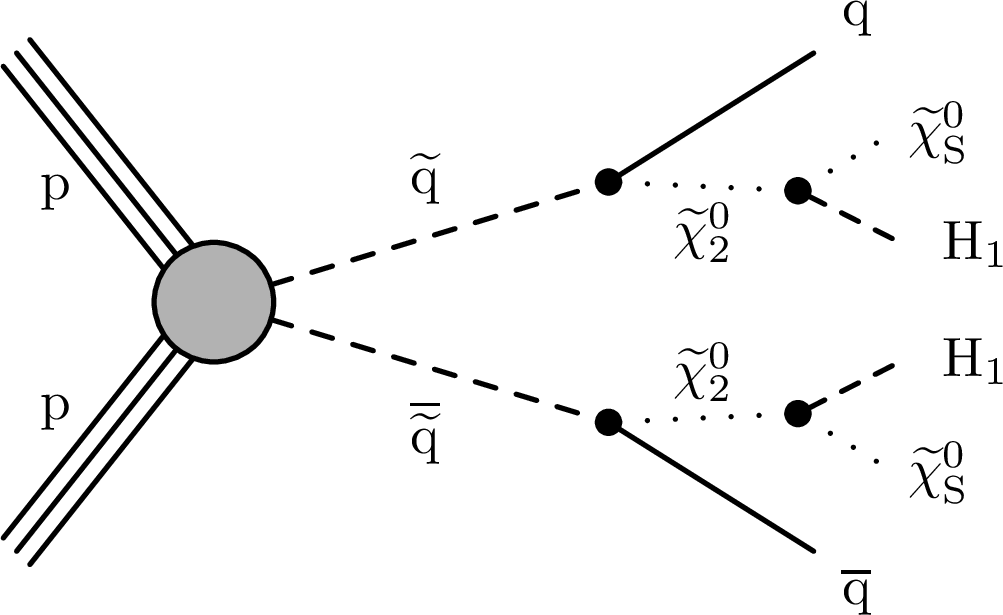
\includegraphics[width=0.5\textwidth]{CMS-PAS-HIG-20-018_Figure_001.png}
        \caption{
            Diagram of squark pair production and subsequent cascade decay. The particle $\tilde{\chi_{2}^{0}}$ is the NLSP,  $\tilde{\chi_{S}^{0}}$ is the singlino-like LSP, and $H_{1}$ is the CP-even singlet-like Higgs boson~\protect\cite{CMS-PAS-HIG-20-018}.
        }
        \label{fig:susy_diagram}
    \end{center}
\end{figure}

The search targets events where both $H_{1}$ bosons decay into $b\bar{b}$ pairs that are reconstructed as large-radius jets, squarks and gluinos with masses $M_{SUSY}$ $\geq$ 1200 GeV and as the branching fraction of $H_{1} \rightarrow b\bar{b}$ decreases for larger $H_{1}$ masses as the WW* and ZZ* decay channels open up, both of which have sizable leptonic branching fractions that become more accessible, therefore the region $M_{{H}_{1}} \leq M_{Z}$ is of most experimental interest. Nevertheless, the search attempts to probe as much of the region  $M_{{H}_{1}} \leq 125$ GeV as possible.
The event pre-selection requires at least two jets jets with a large opening angle corresponding to R = 0.8
(AK8 jets), wide-angle soft radiation is recursively removed from the jet. If there are more than two
candidate AK8 jets, the two with the highest double-b-tag discriminator values are selected
as those most likely originating from $H_{1} \rightarrow b\bar{b}$ decays. %The two selected AK8 btagged jets randomly assigned the labels 'A' and 'B' further their soft-drop masses define a 2D parameter space of the search.

No evidence is found for any excess of events beyond the background expectations of the SM. $H_{1}$ bosons arising from the decays of squarks or gluinos, with masses in the range 40–120 GeV are excluded at the 95$\%$ confidence level, the same for SUSY masses in the range 1200-2500 GeV, are excluded at the 95$\%$ confidence level, as reported in Fig.~\ref{fig:limits_susy}.

\begin{figure}[!htb]
    \begin{center}
        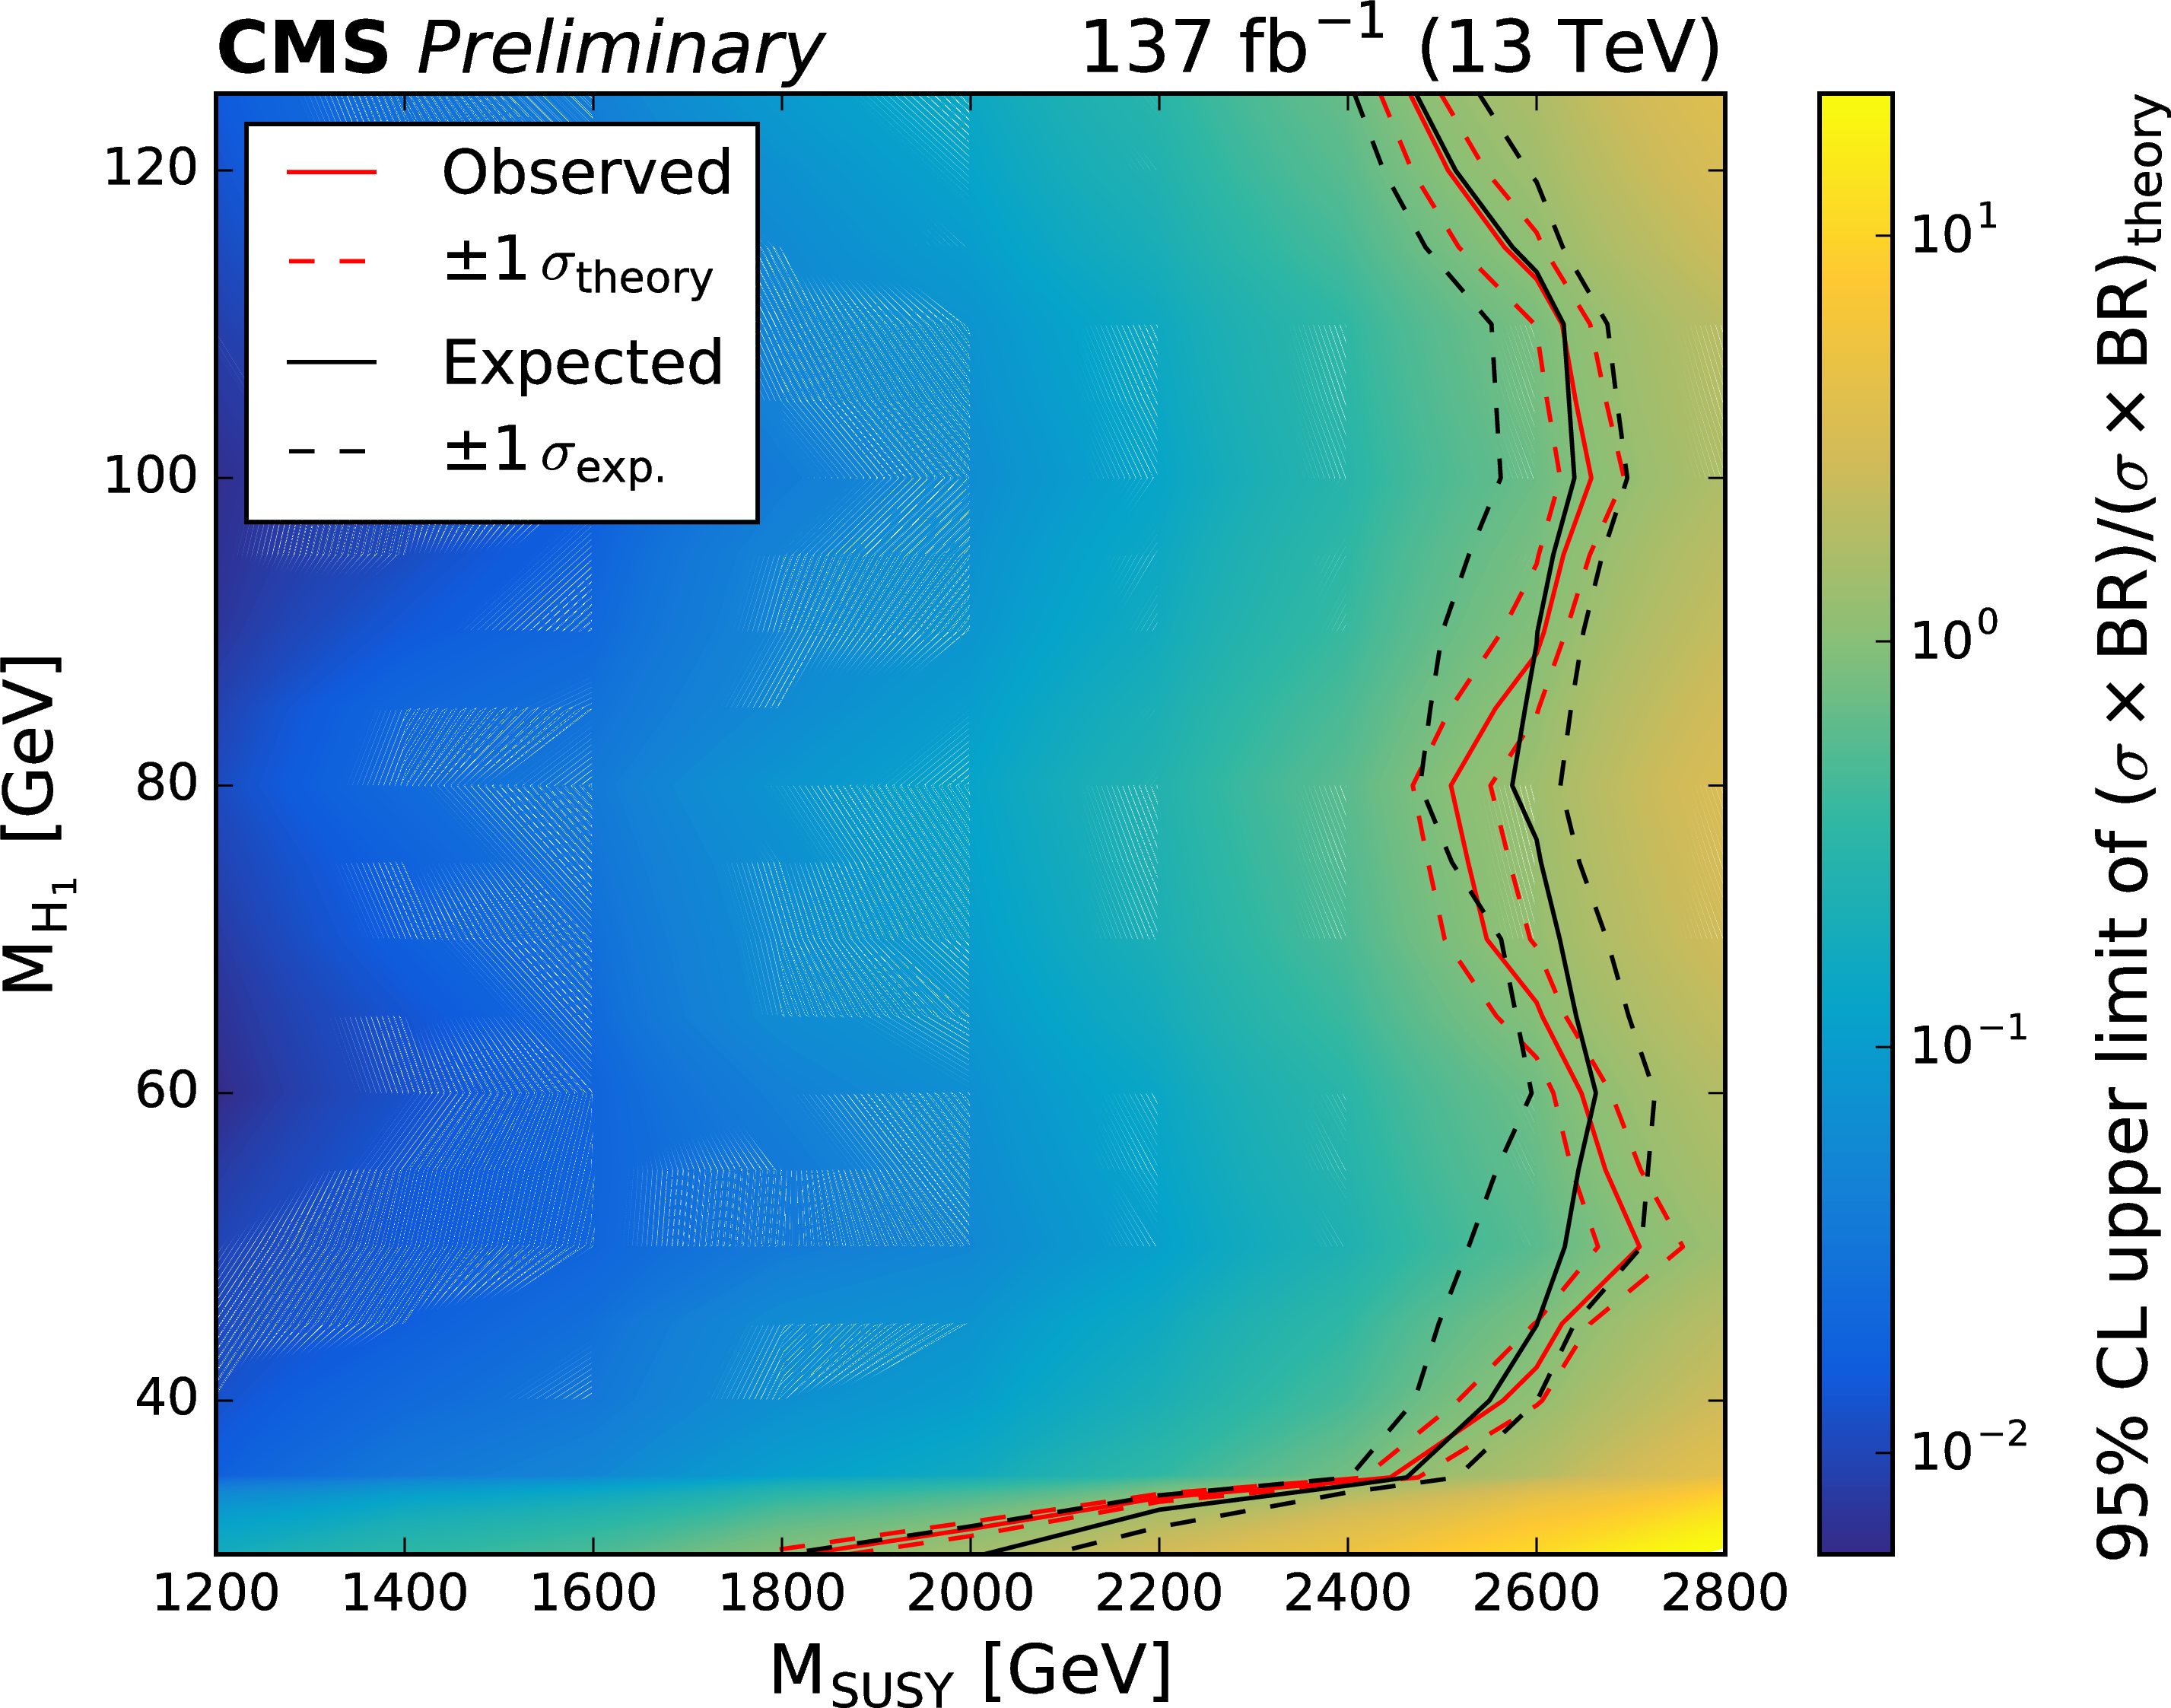
\includegraphics[width=0.5\textwidth]{CMS-PAS-HIG-20-018_Figure_010.png}
        \caption{
            The observed 95$\%$ CL upper limit of ($\sigma$ x BR)/($\sigma$ x BR)theory (indicated by the colour scale) as a function of $H_{1}$ and $M_{SUSY}$. The solid red (black) line delineates the observed (median expected) excluded region. The dashed red (black) line delineates the observed (expected) excluded regions with $\pm1\sigma$ in theoretical (experimental) uncertainty~\protect\cite{CMS-PAS-HIG-20-018}.
        \label{fig:limits_susy}
         }
    \end{center}
\end{figure}
%%%%%%%%%%%%%%%%%%%%%%%%%%%%%%%%%%%%%%%%%%%%%%%%%%%%%%%%%%%%%%%%%%%%%%%%%%%
\subsection\protect{Search for a heavy Higgs boson decaying into two lighter Higgs bosons in the $\tau\tau bb$ final state}

Many searches for additional Higgs bosons in the context of the MSSM have been performed by
the LHC experiment. In the absence of signal, these have led to the exclusion of large parts of the MSSM parameter space for masses of the additional neutral Higgs bosons up to $\approx$ 2 TeV~\cite{PhysRevLett.125.051801}. 
On the other hand, the parameter space of the NMSSM, is still largely unconstrained~\cite{PhysRevD.90.095014}.

The reported search~\cite{CMS:tautaubb} focuses on heavy Higgs boson H decaying to the observed Higgs boson h(125 GeV) and an additional scalar $h_{S}$ with a requirement of mass $( m_{h_{S}} < m_{H} - m_{h} )$.
Restricted to H production from gluon fusion ( Fig.~\ref{fig:diagrams_tautaubb}) the search explores high mass ranges; 240-3000 GeV for $m_{H}$ and 60-2800 GeV for $m_{h_{S}}$. The h and $h_{S}$  bosons are required to decay into a pair of $\tau$ leptons and a pair of $b$ quarks, respectively. The decay of the Higgs bosons h into tau leptons is favored for its cleaner signature compared to the decay into b quarks. The decay of the additional scalar $h_{S}$ into b quarks is chosen for its large branching fraction.
\begin{figure}[!htb]
    \begin{center}
        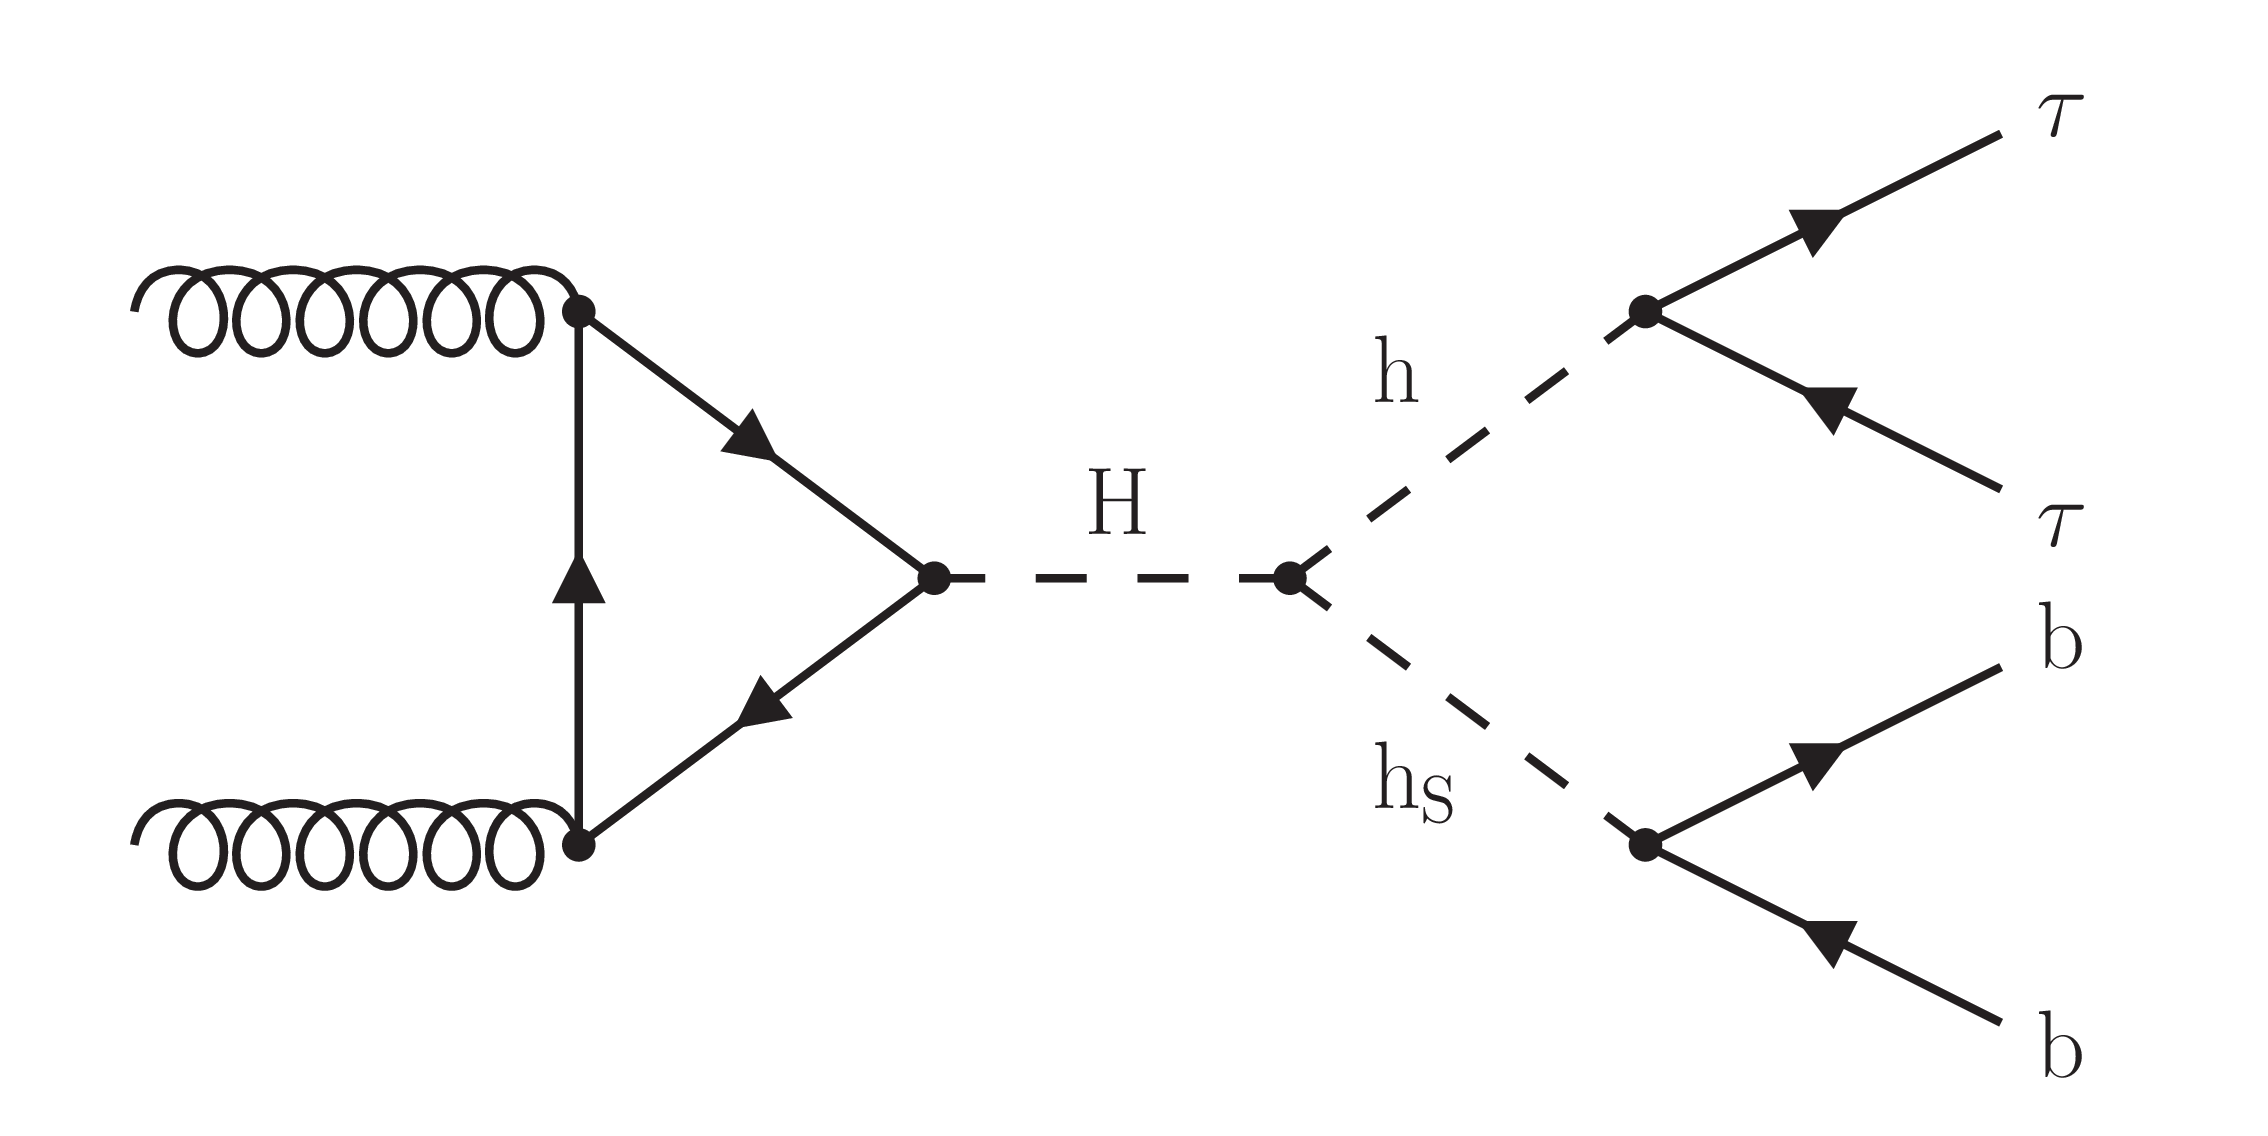
\includegraphics[width=0.5\textwidth]{CMS-HIG-20-014_Figure_001.png}
        \caption{
           Feynman diagram of the $gg \rightarrow H \rightarrow h(\rightarrow \tau\tau)h_{S}(\rightarrow bb)$ process~\protect\cite{CMS:tautaubb}.
        }
        \label{fig:diagrams_tautaubb}
    \end{center}
\end{figure}
The event selection is based on the presence of a single electron or muon, an $e\tau_{h}$ or $\mu\tau_{h}$ pair, or a $\tau_{h}\tau_{h}$ pair. %The overall normalization of all backgrounds is constrained by dedicated event categories, obtained from neural network (NN) multi-classification, 

A summary of the observed limits 95$\%$CL for wide range of pairs of $m_{H}$ and $ m_{h_{S}}$ is shown in Fig.~\ref{fig:limits_tautaubb}.
\begin{figure}[!htb]
    \begin{center}
        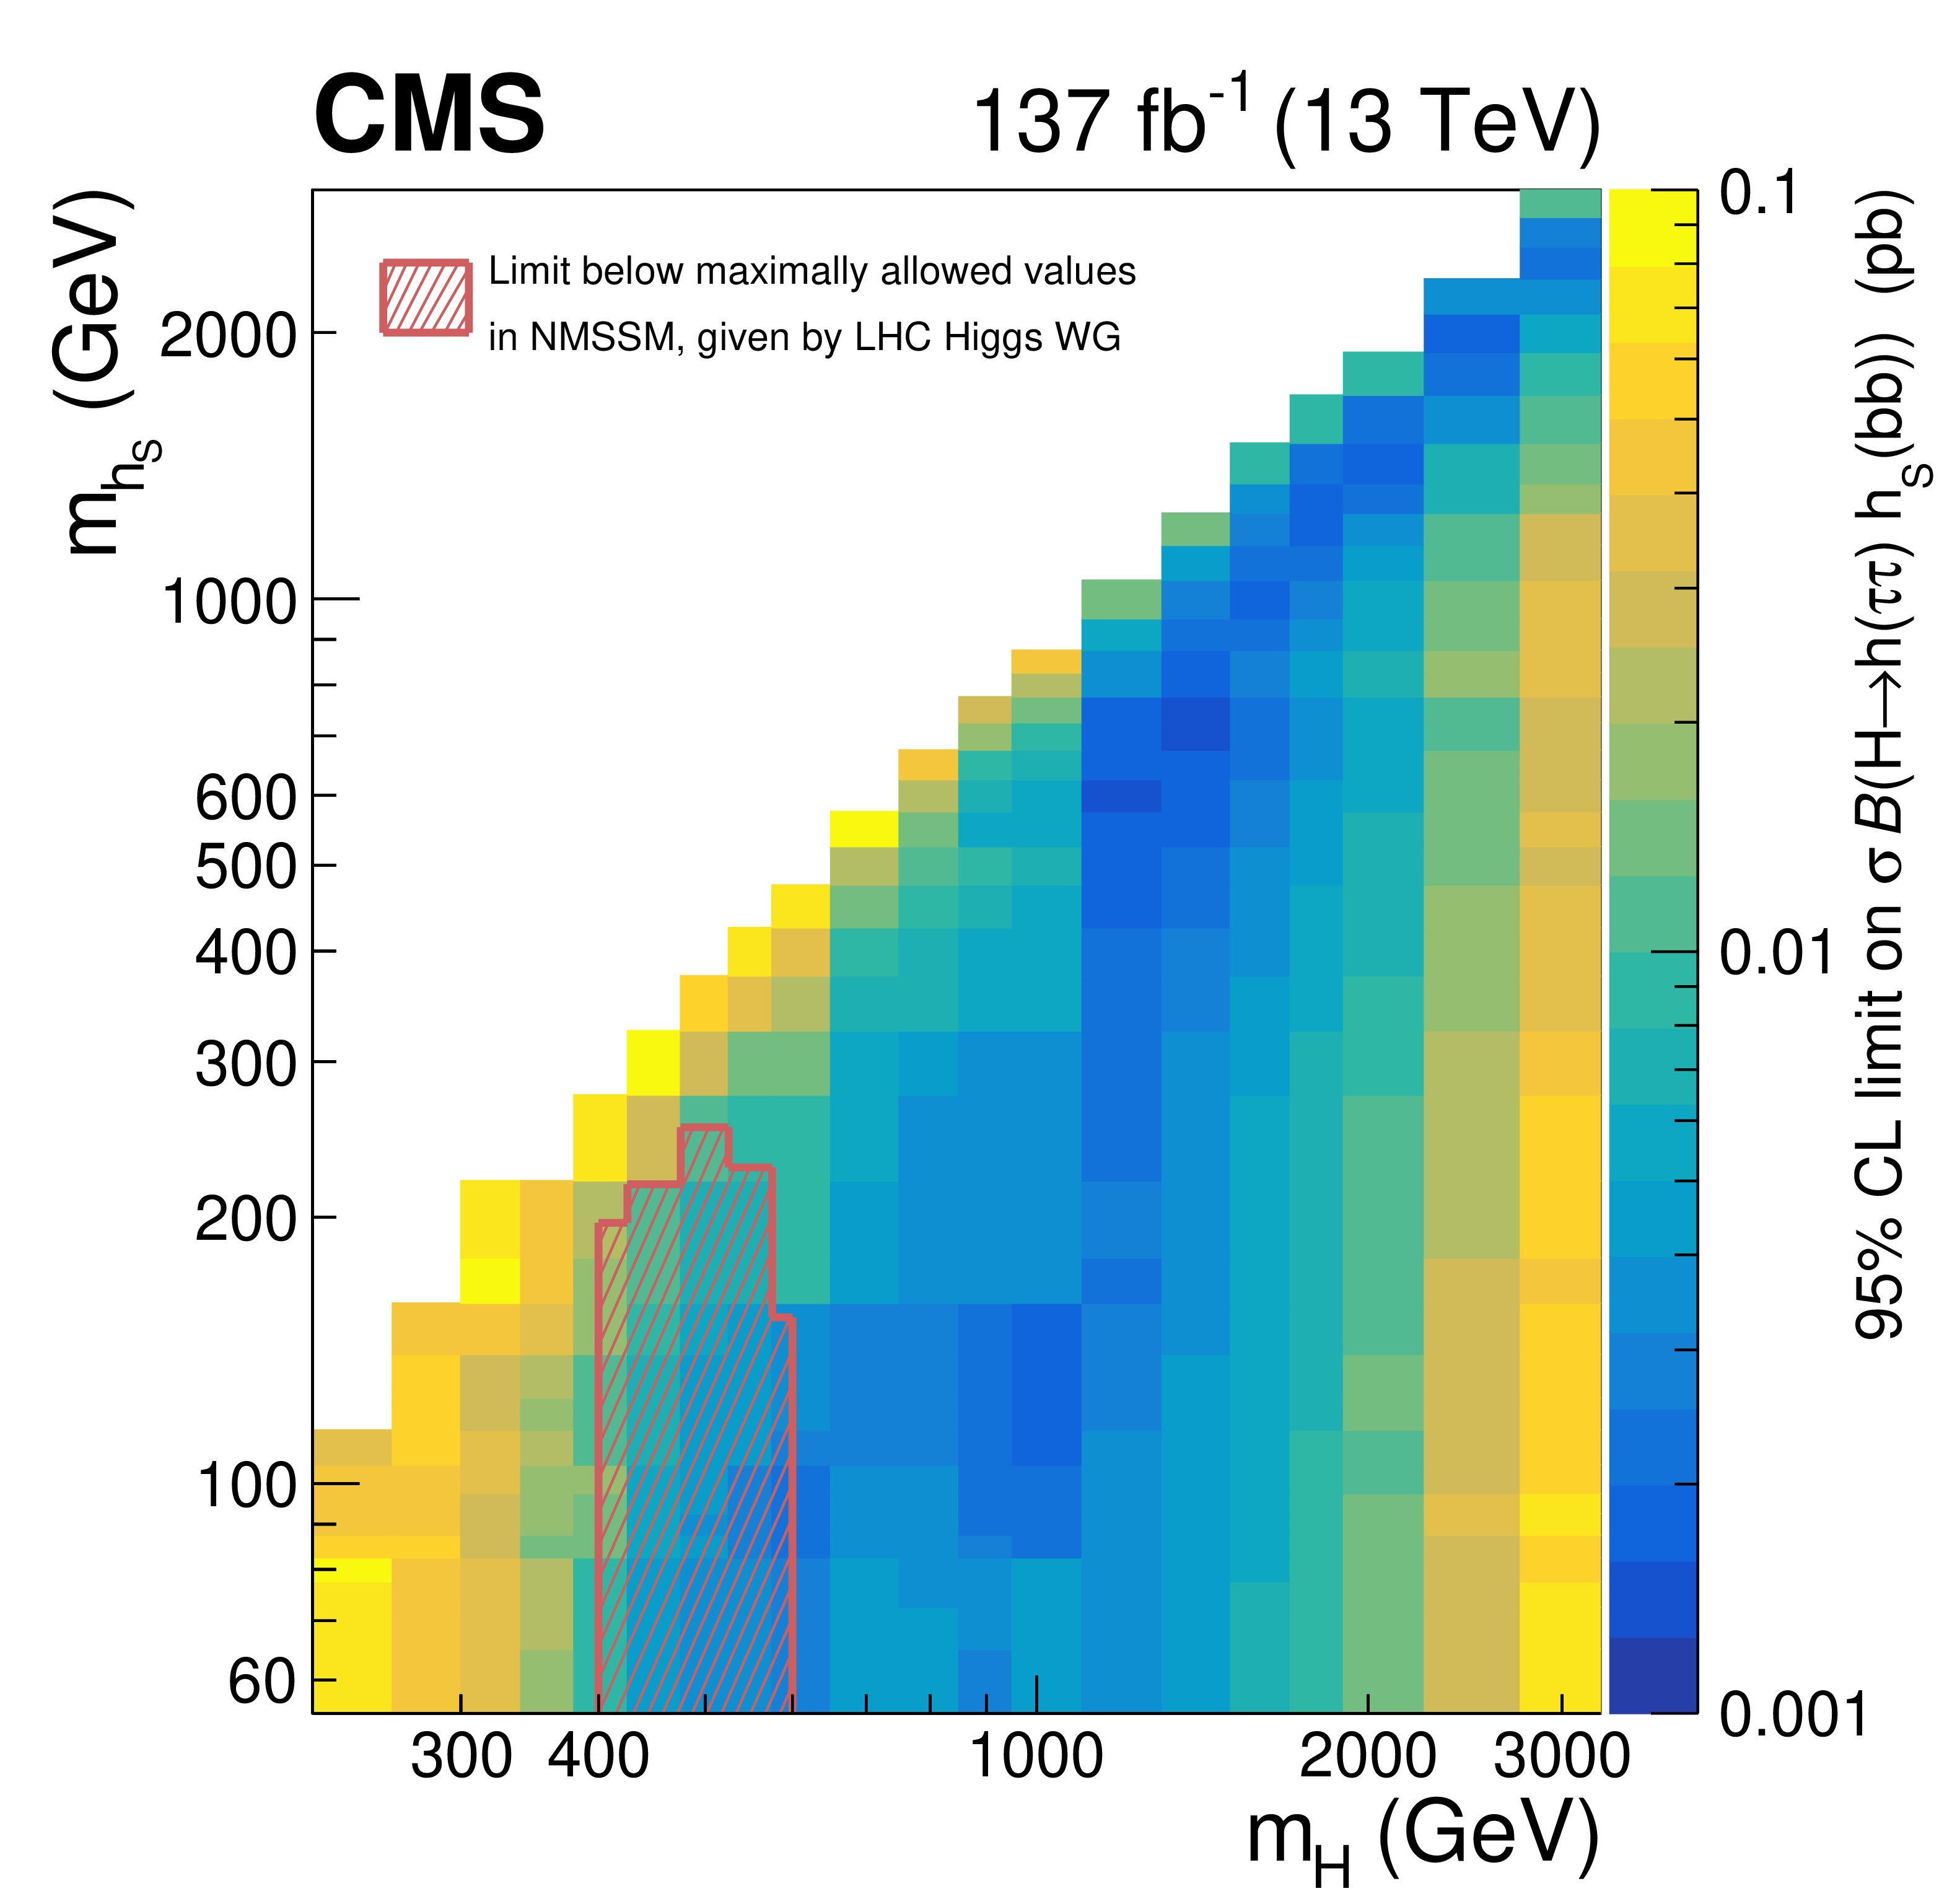
\includegraphics[width=0.5\textwidth]{CMS-HIG-20-014_Figure_006.png}
        \caption{
           Summary of the observed limits on $\sigma B(H \rightarrow (\tau_{h}\tau_{h})h_{S}(b\bar{b}))$~\protect\cite{CMS:tautaubb}.
        }
        \label{fig:limits_tautaubb}
    \end{center}
\end{figure}
% \ \\[1cm]
\vspace{2cm}
%\clearpage
%%%%%%%%%%%%%%%%%%%%%%%%%%%%%%%%%%%%%%%%%%%%%%%%%%%%%%%%%%%%%%%%%%%%%%%%%%%
%%\subsection{Search for a heavy Higgs boson decaying to a pair of W bosons}
%% it is a search based on 2016 data, won't be covered here
%%%%%%%%%%%%%%%%%%%%%%%%%%%%%%%%%%%%%%%%%%%%%%%%%%%%%%%%%%%%%%%%%%%%%%%%%%%
\subsection{Exotic decays of the Higgs boson}\label{subsec:exo}

Decays of the type H $\rightarrow$ aa, where a is a light pseudoscalar boson, are well motivated in various Beyond the Standrd Model (BSM) scenarios. In many scenarios, the branching fraction of the pseudoscalars to a pair of photons is sufficient to be visible at the LHC. The final state with four photons provides an experimental signature that has very low contributions from SM processes and, is therefore an important channel to pursue a search for light pseudoscalars.

A previous search for light pseudoscalars in events with at least three photons was performed by the ATLAS collaboration using the LHC data collected at $\sqrt{s}$= 8 TeV~\cite{4gamma_atlas}. Recently a model-independent search by the CMS collaboration has been performed for exotic decays of the observed Higgs boson to a pair of light pseudoscalars that range in mass from 15 to 60 GeV, each of which subsequently decay to a pair of photons~\cite{CMS-PAS-HIG-21-003}. A Feynman diagram contributing to this
process at leading-order (LO) is shown in Fig.~\ref{fig:exo_diagrams}.
 %

 \begin{figure}[!htb]
    \begin{center}
        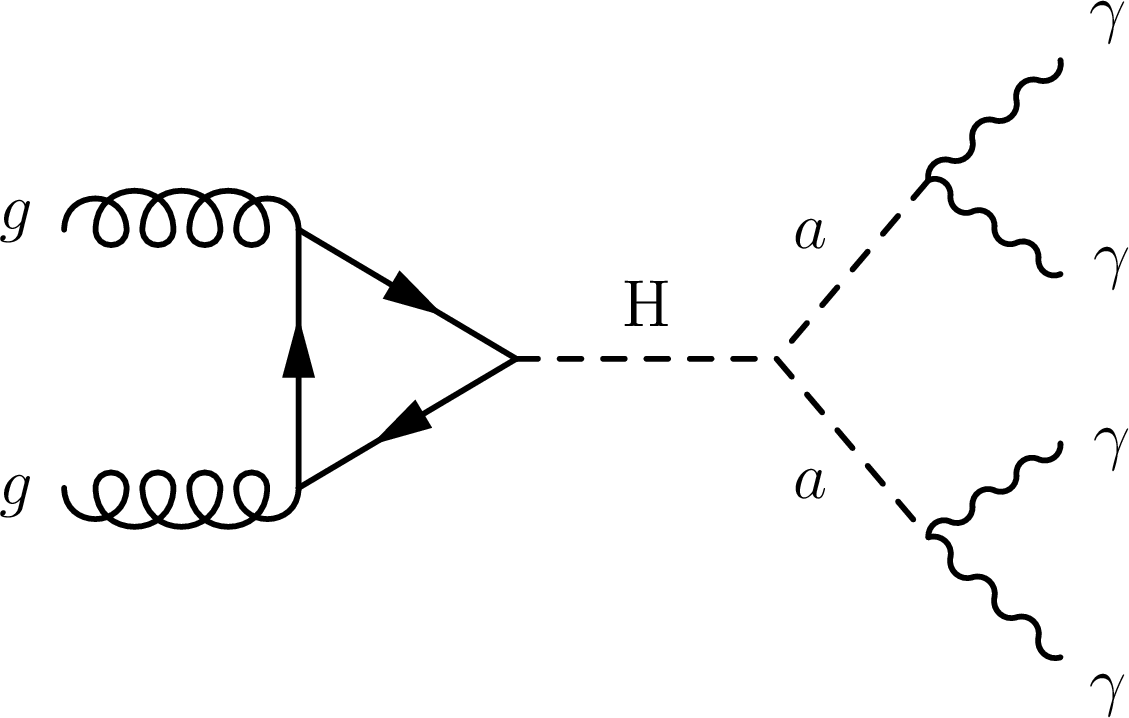
\includegraphics[width=0.4\textwidth]{CMS-PAS-HIG-21-003_Figure_001.png}
        \caption{
             Feynman diagram for BSM decay of the Higgs boson into a pair of light pseudoscalars, which further decay to photons~\protect\cite{CMS-PAS-HIG-21-003}.
        }
        \label{fig:exo_diagrams}
    \end{center}
\end{figure}

The dominant backgrounds in this search~\cite{CMS-PAS-HIG-21-003} are SM produced $\gamma\gamma$ + jets, $\gamma$+ jets, as well as multijet events, where jets are misidentified as isolated photons. Because of the low signal selection efficiency on the background samples, it is difficult to model
the background from simulation. The expected background model, which is used to train an
event classifier, is estimated from data. The method, referred to as event mixing, which aims at estimating the background contribution using the original data set as input. While, the signal model is constructed from a parametric fit to the simulated signal.

No significant deviation from the background-only hypothesis is observed, and upper limits are set on the product of the Higgs boson production cross section and branching fraction into four photons~\cite{CMS-PAS-HIG-21-003}.
\begin{figure}[!htb]
    \begin{center}
        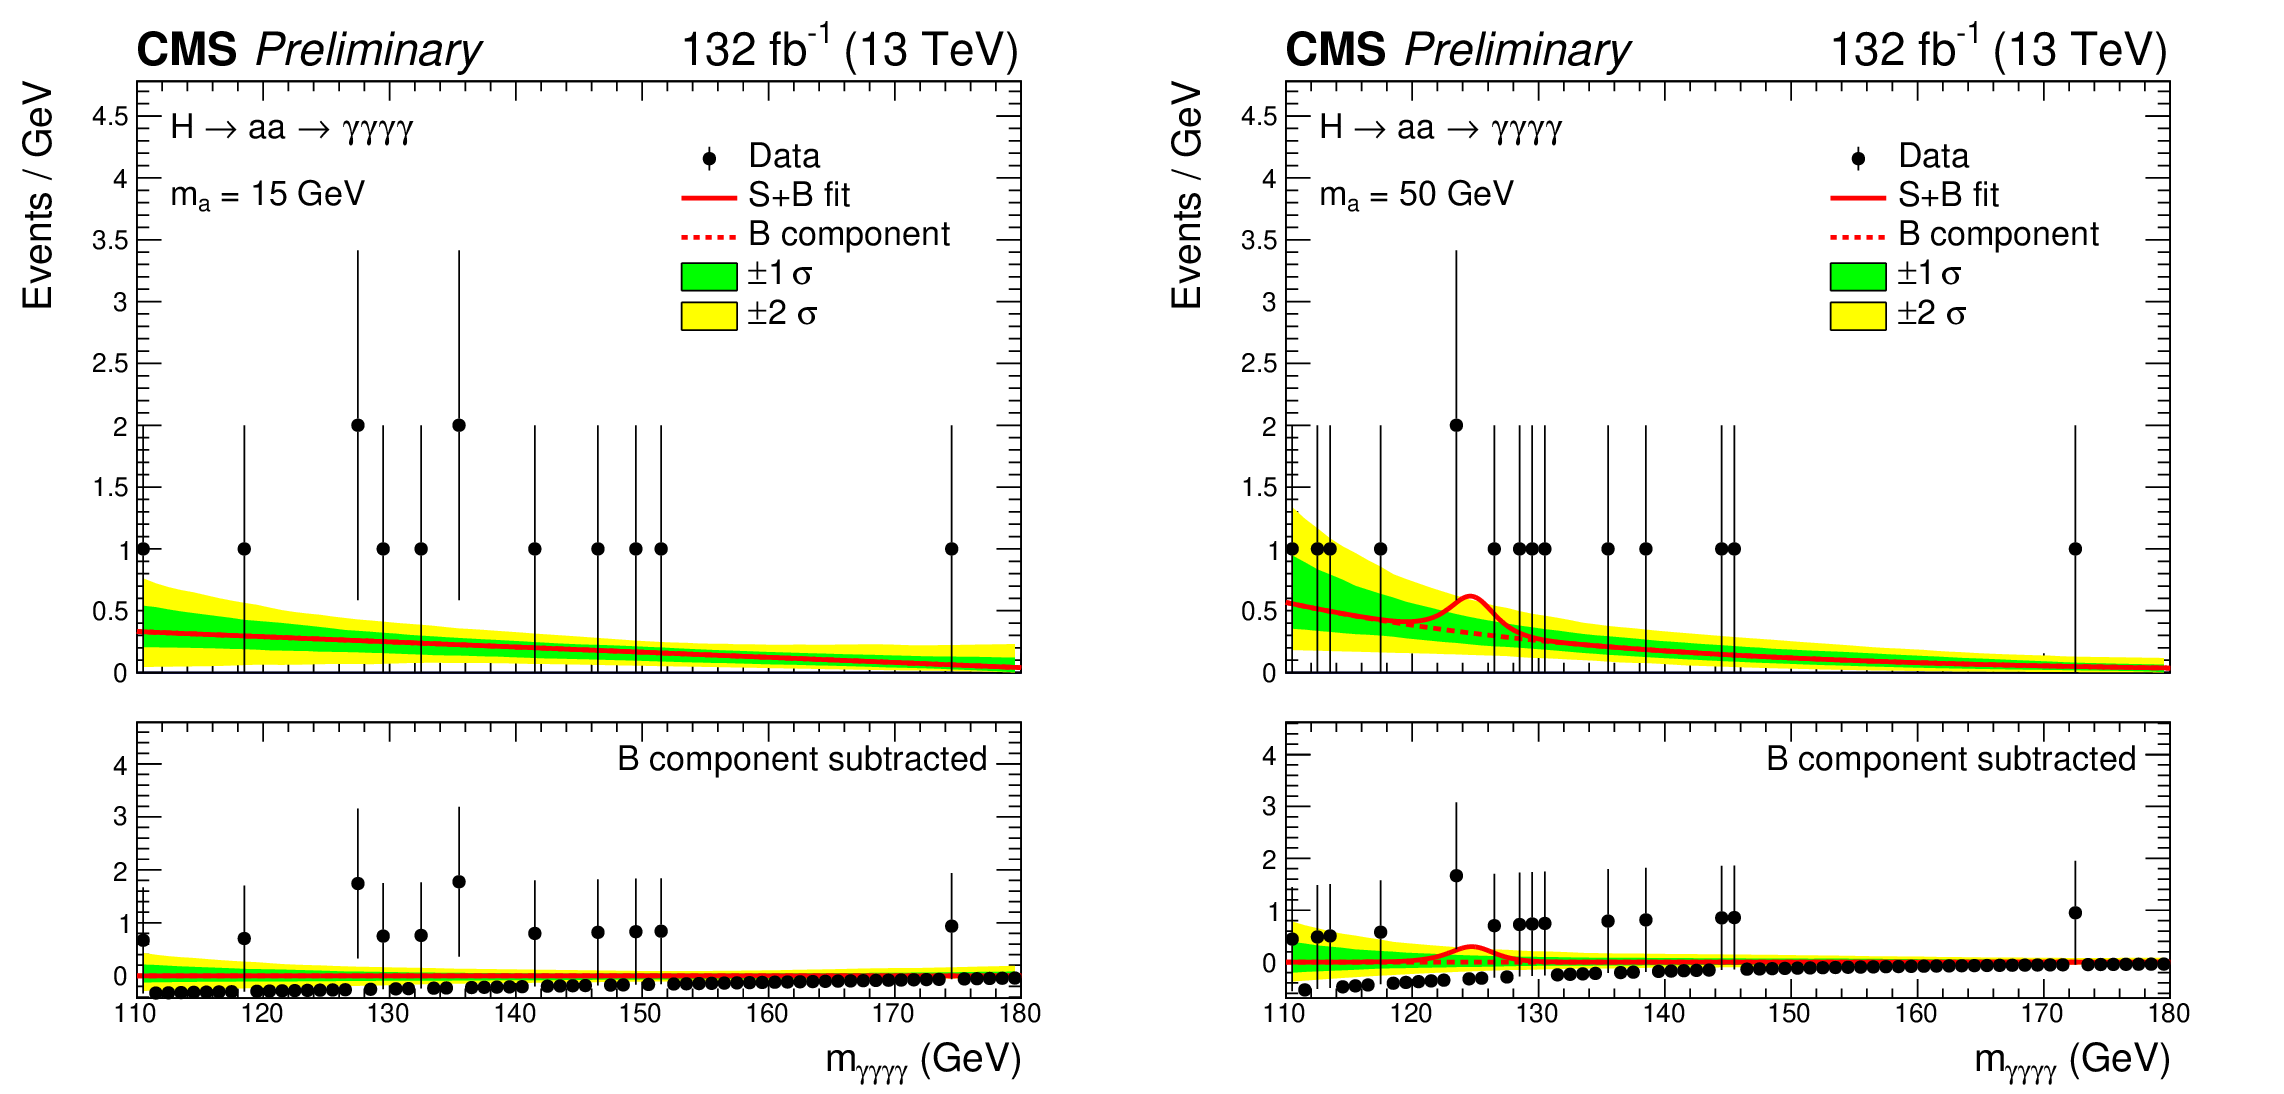
\includegraphics[width=0.8\textwidth]{CMS-PAS-HIG-21-003_Figure_006.png}
        \caption{
           Invariant mass distribution, $m_{\gamma\gamma\gamma\gamma}$, for data (black points) and signal-plus-background model fit is shown for $m_{a}$= 15 GeV (left) and $m_{a}$= 50 GeV (right). The solid red line shows the total signal-plus-background contribution, whereas the dashed red line shows the background component only. The lower panel in each plot shows the residual signal yield after the background subtraction~\protect\cite{CMS-PAS-HIG-21-003}.
        }
        \label{fig:exo_limits}
    \end{center}
\end{figure}
%\clearpage
%%%%%%%%%%%%%%%%%%%%%%%%%%%%%%%%%%%%%%%%%%%%%%%%%%%%%%%%%%%%%%%%%%%%%%%%%%%
\section{Extended charged Higgs searches}

At the LHC, interactions from vector boson scattering (VBS) are characterized by the presence of two gauge bosons in association with two forward jets with a large pseudorapidity separation ($|\Delta\eta_{ij}|$) and a large dijet invariant mass ($m_{jj}$).
Extended Higgs sectors that include only electroweak doublets with SM like quantum
numbers, as in MSSM, automatically preserve custodial
symmetry~\cite{Low:2010jp} regardless of whether each doublet obtains the same vacuum expectation
value or not. The Georgi-Machacek model (GM) adds scalar triplets to the Standard Model Higgs sector in such a way as to preserve custodial SU(2) symmetry in the scalar potential. This allows the triplets to have a non-negligible vacuum expectation value~\cite{Vega2017TheSG}.

\subsection{Search for charged Higgs bosons produced in vector boson fusion processes and decaying into vector boson pairs}
The Georgi-Machacek (GM) model contains singly- and doubly-charged Higgs particles that couple
to vector boson pairs at tree level, leading to $H_{5}^{+} \rightarrow W^{+} Z$ and like-sign $H_{5}^{++} \rightarrow W^{+}W^{+}$ signatures.
Fig.~\ref{fig:Georgi_diagrams} shows representative Feynman diagrams for the production and decay of the charged Higgs bosons.

Recently the CMS collabortaion performed a search~\cite{CMS:2021wlt} for these signatures in the leptonic decay modes $W^{+}W^{+} \rightarrow l^{\pm}\nu l^{\pm}\nu$ and $W^{\pm}Z \rightarrow l^{\pm}\nu l^{\mp}\nu$, where $l= e, \mu$.
In the GM model, the production and decays of the $H_{5}$ states depend on the two parameters $mH_{H_{5}}$ and $s_{H}^{2}$, where $s_{H}^{2}$ characterizes the fraction of the W boson mass squared generated by the vacuum expectation value of the triplet fields. No excess of events with respect to the SM background predictions is observed. The most stringent limits to date derived at 95$\%$ confidence level are reported in Fig.~\ref{fig:Georgi_limits} on the product of the cross section and branching fraction for vector boson fusion production of charged Higgs bosons decaying into vector bosons in mass ranges from 200 to 3000 GeV.

 \begin{figure}[!htb]
    \begin{center}
        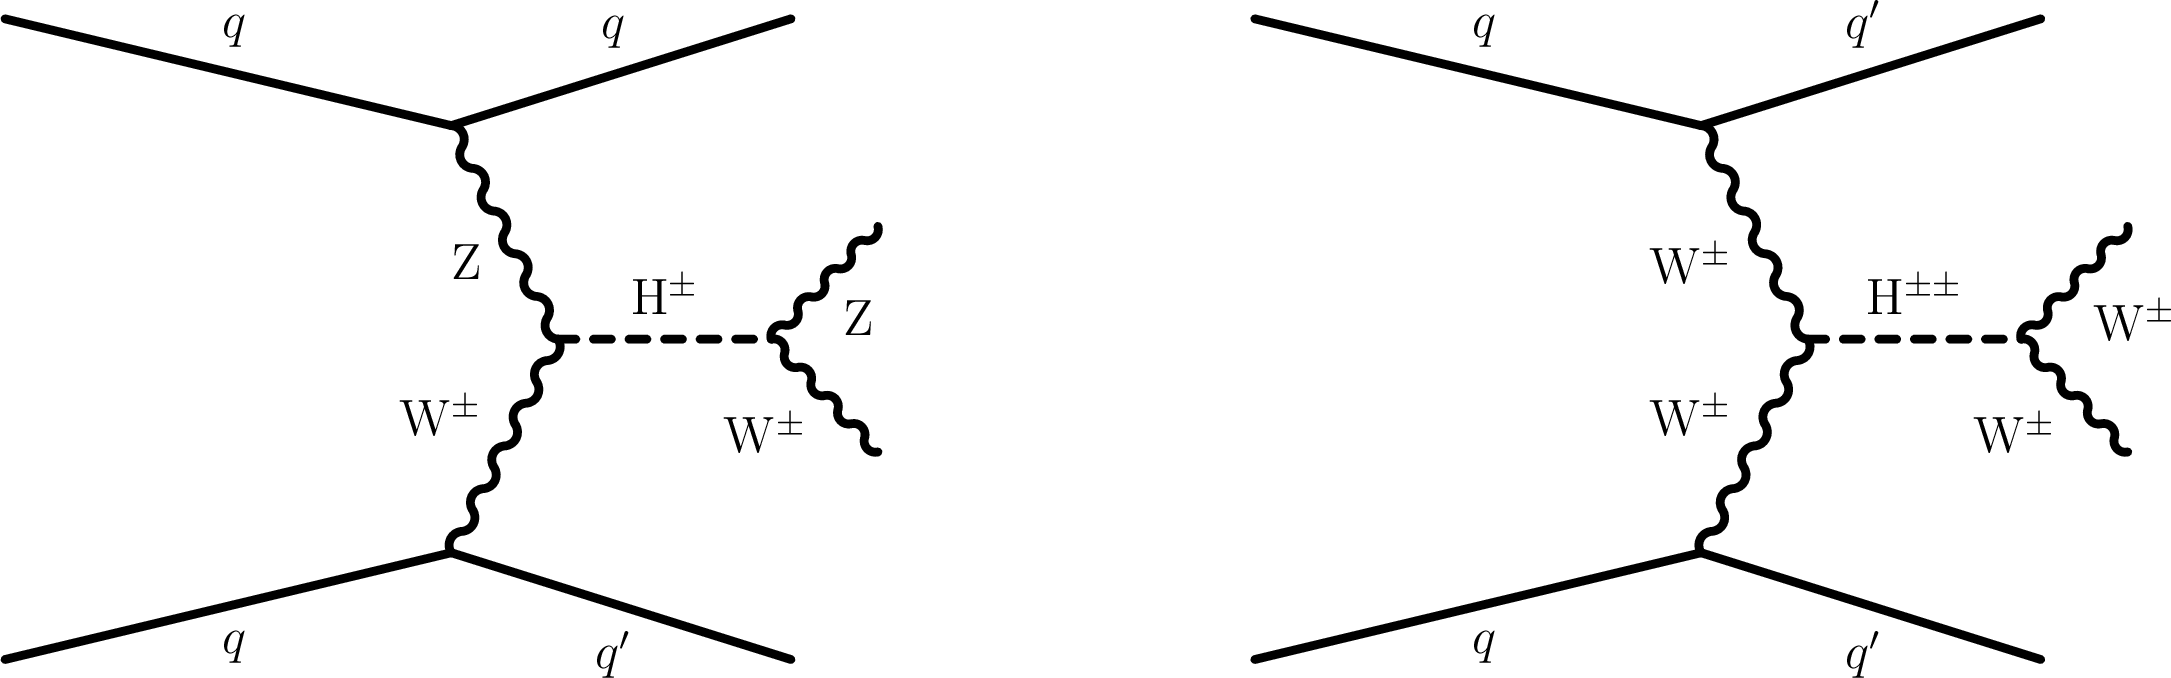
\includegraphics[width=0.6\textwidth]{CMS-HIG-20-017_Figure_001.png}
        \caption{
              Examples of Feynman diagrams showing the production of singly (left) and doubly (right) charged Higgs bosons via VBF~\protect\cite{CMS:2021wlt}.
        }
        \label{fig:Georgi_diagrams}
    \end{center}
\end{figure}

 \begin{figure}[!htb]
    \begin{center}
        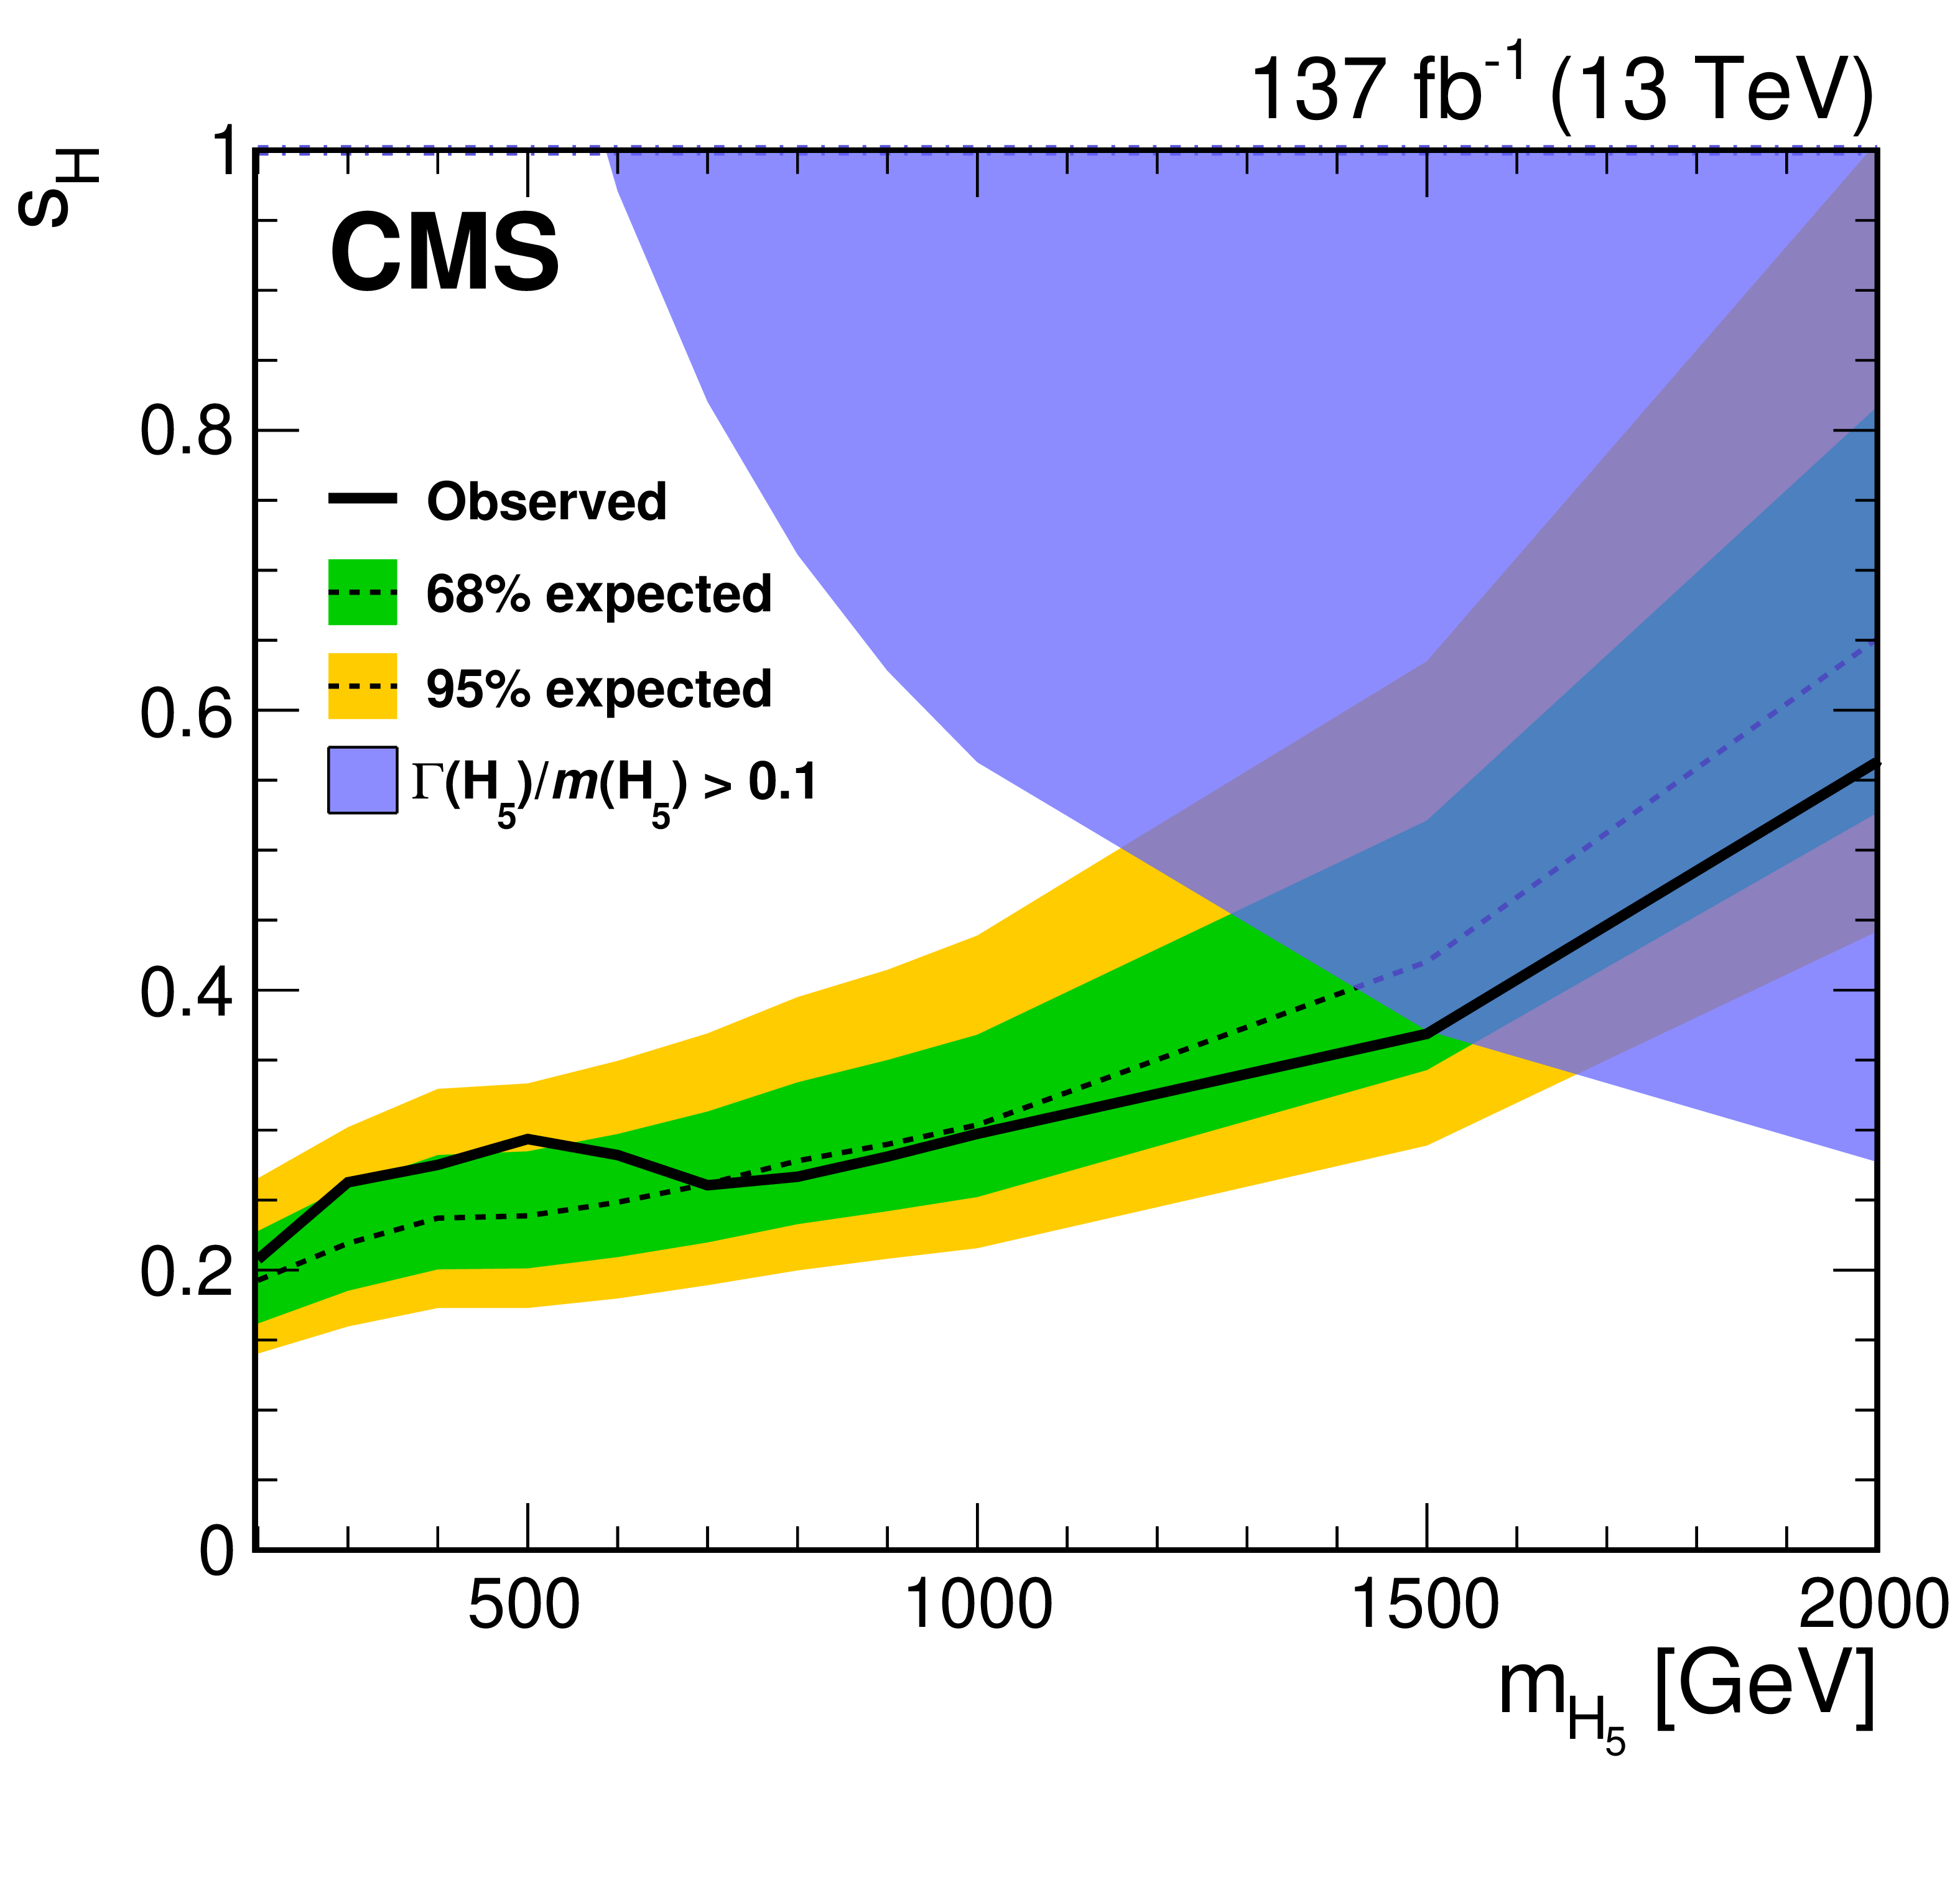
\includegraphics[width=0.5\textwidth]{CMS-HIG-20-017_Figure_008-c.png}
        \caption{
              Expected and observed exclusion limits at 95$\%$ CL for $s_{H}$ as functions of $H_{H_{5}}$ in the GM model~\protect\cite{CMS:2021wlt}.The exclusion limits for $s_{H}$ are shown up to $m_{H_{5}}$= 2000 GeV, given the low sensitivity in the GM model for values above that mass. Values above the curves are excluded.
        }
        \label{fig:Georgi_limits}
    \end{center}
\end{figure}
%\clearpage
%%%%%%%%%%%%%%%%%%%%%%%%%%%%%%%%%%%%%%%%%%%%%%%%%%%%%%%%%%%%%%%%%%%%%%%%%%%
% \ \\[2cm]
%\vspace{2cm}
\section{Summary}
During run 2, the LHC has provided an integrated luminosity of 137 $fb^{-1}$. Despite the increase in precision, the LHC data have so far not given any indications of the couplings
being different from the predicted ones in the SM.
Direct searches for additional Higgs bosons have been conducted in a wide variety of channels together with indirect approaches through precision measurements which represent a valuable, complementary way to reach the ultimate goal of finding new physics. Despite the fact that there is no significant excess observed beyond the standard model expectation, still a remarkable improvement in search strategies and in object reconstruction, as demonstrated in several of the discussed searches, allowing to set stronger constraints on the parameters of BSM models.
To this end, a sign that masses of new particles might be lying at very high energy scales underlines once again the high importance of the High-Luminosity LHC project.
%%%%%%%%%%%%%%%%%%%%%%%%%%%%%%%%%%%%%%%%%%%%%%%%%%%%%%%%%%%%%%%%%%%%%%%%%%%
%\section*{Acknowledgments}
%%%%%%%%%%%%%%%%%%%%%%%%%%%%%%%%%%%%%%%%%%%%%%%%%%%%%%%%%%%%%%%%%%%%%%%%%%%
\section*{References}
\bibliography{blois.bib}
%%%%%%%%%%%%%%%%%%%%%%%%%%%%%%%%%%%%%%%%%%%%%%%%%%%%%%%%%%%%%%%%%%%%%%%%%%%
\end{document}
%%%%%%%%%%%%%%%%%%%%%%
% End of blois.tex   %
%%%%%%%%%%%%%%%%%%%%%%
\vspace{2cm}